\section{Forstærker}
Beskrivelse af forstærker \\
Fra INA114 databladet ses en formel til udregning af komponentværdier for at skabe den ønskede gain. Da vi ønsker en gain på 640 udregnes komponentværdierne til følgende:

\subsection{Beregninger}
\vspace{0.5 cm}
\[ sensitivity = 5\cdot\frac{µV}{V\cdot mmHg} \]
\[ powersupply = 5V \]
\[ maximumPressure = 250 mmHg \]
\[ V_{out} =5\cdot\frac{µV}{V\cdot mmHg} \cdot 5V \cdot 250 mmHg = 6250 µV \]
\[ V_{out} =6,25 mV \]
\[ gain = \frac{4V}{V_{out}} = 640 \]
\[ G = 1+\frac{50k\Omega}{R_{G}} \]
\[ 640 = 1+\frac{50k\Omega}{R_{G}} \rightarrow R_{G}=\frac{5000}{639}\]
\[ R_{G} = 78,247 \Omega \]

Med ovenstående beregninger vurderes det, at vi skal bruge en modstand på ca. 78$\Omega$ for at forstærke signalet 640 gange.

\vspace{0.5 cm}

\subsection{Test af forstærker med spændingsdeler}
\vspace{0.2 cm}
For at teste forstærkerens virkning bruges en spændingsdeler til at gøre en spænding fra Analog Discovery mindre. Vi ønsker at teste, om forstærkeren forstærker signalet 640 gange. Komponenterne til spændingsdeleren udregnes til følgende:

Tilfældig modstand vælges
\[ R2=100 k\Omega \]

Tilfældig spænding vælges
\[ V1 = 4V \]

Ønsket nedforstærkning
\[ V2=0,00625V\]

R1 bestemmes:
\[ 0,00625V = 4V\cdot \frac{R1}{R1+R2}\rightarrow R1 = 156,4945 \Omega\]

Spændingsdeleren blev tilsluttet systemet, og vi sendte 4 V igennem. Der blev målt på udgangen af forstærkeren, hvilket vi forventede at være 640 gange større end spænding efter spændingsdeleren. 
\clearpage


\subsection{Test af forstærker med vandsøjle}
For at kunne teste forstærkeren på vandsøjlen måtte vi tage tryktransduceren i brug. Transduceren blev erstattet med spændingsdeleren, samt tilsluttet vandsøjlen.
Der blev udført en række tests med tryk på henholdsvis:

0 mmHg
10 mmHg
50 mmHg
100 mmHg

\begin{figure}[h!]
	\centering
	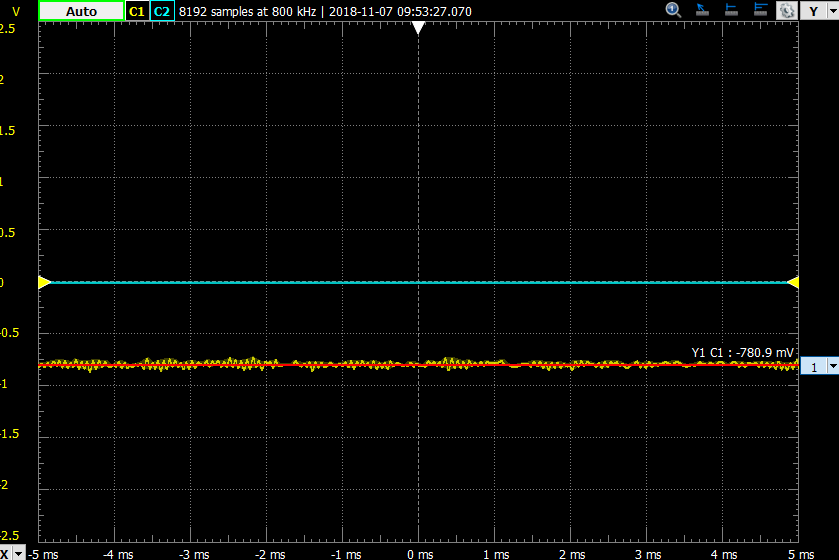
\includegraphics[width=1\linewidth]{Hardware/0mmHg}
	\caption{Spændning ved atmosfærisk tryk}
	\label{fig:0mmHg}
\end{figure}

\begin{figure}[h!]
	\centering
	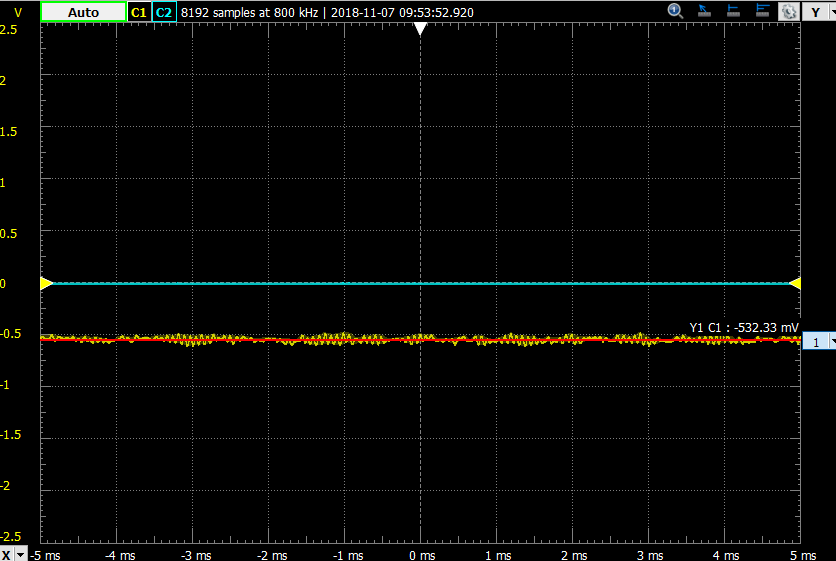
\includegraphics[width=1\linewidth]{Hardware/10mmHg}
	\caption{Spændning ved 10 mmHg}
	\label{fig:10mmHg}
\end{figure}

\begin{figure}[h!]
	\centering
	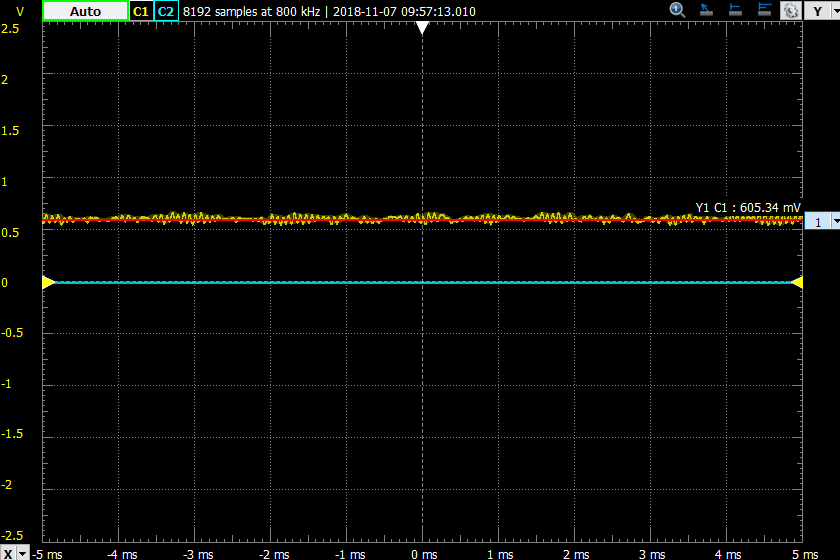
\includegraphics[width=1\linewidth]{Hardware/50mmHg}
	\caption{Spændning ved 50 mmHg}
	\label{fig:50mmHg}
\end{figure}

\begin{figure}[h!]
	\centering
	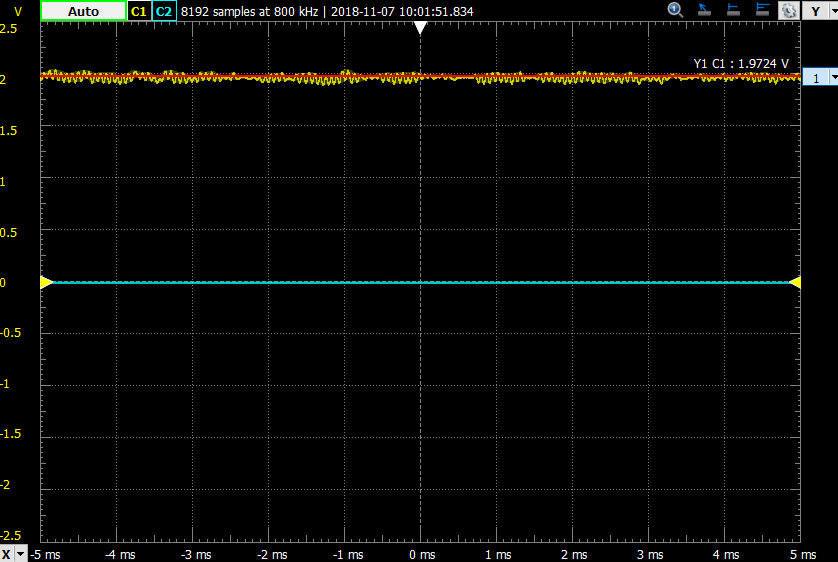
\includegraphics[width=1\linewidth]{Hardware/100mmHg}
	\caption{Spændning ved 100 mmHg}
	\label{fig:100mmHg}
\end{figure}

De målte spændinger er blevet plottet, som funktion af tryk.

\begin{figure}[h!]
	\centering
	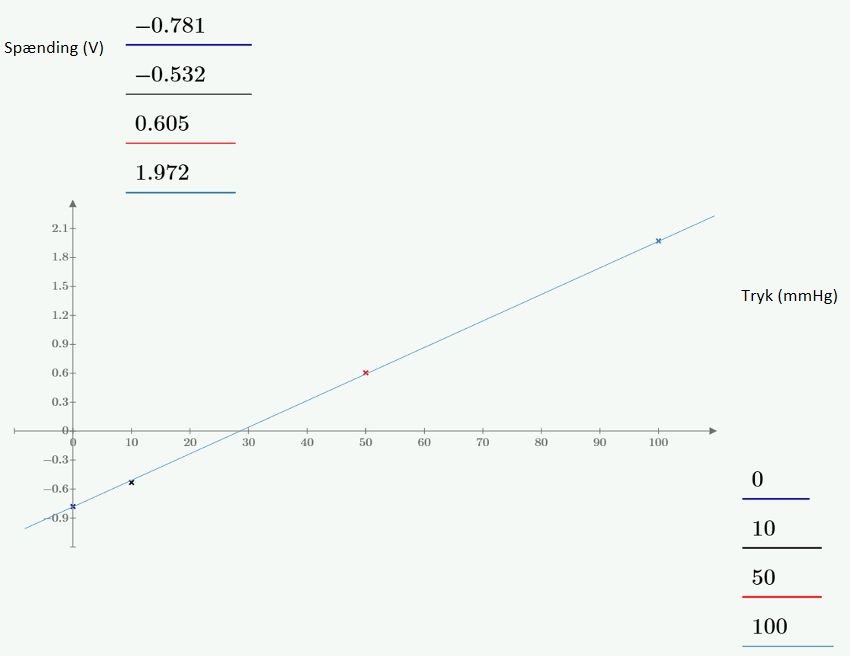
\includegraphics[width=1\linewidth]{Hardware/GrafTrykOgSpaending}
	\caption{Spænding som funktion af tryk}
	\label{fig:GrafTrykOgSpaending}
\end{figure}

Der ses en tydelig sammenhæng mellem spænding og tryk, og antager vi at denne sammenhæng forsætter kan vi opsætte regnestykket:

250 mmHg  / 100 mmHg = 2,5
1,972 V * 2,5 = 4,93 V
4,93 V - 0,781 V = 4,149 V

Vi ved udfra tidligere beregninger at vi forventer at vi ved et tryk på 250 mmHg vil opnå en spændining på 4 V, hvilket stemmer godt overens med vores test.

\clearpage

